\documentclass[11pt]{standalone}
\usepackage{amssymb} 
\usepackage{amsmath} 
\usepackage[no-math]{fontspec}
\usepackage{unicode-math}
\setmainfont{TeX Gyre Heros}
\setmathfont{Stix Two Math}
\usepackage{xcolor}
\usepackage{tikz}
\usetikzlibrary{arrows.meta, backgrounds}
\definecolor{myblue}{HTML}{1E3A8A}
\definecolor{lightblue}{HTML}{BFDBFE}
\definecolor{bgcolor}{HTML}{E5E7EB}
\definecolor{highlight}{HTML}{CCDEE9}
\begin{document}
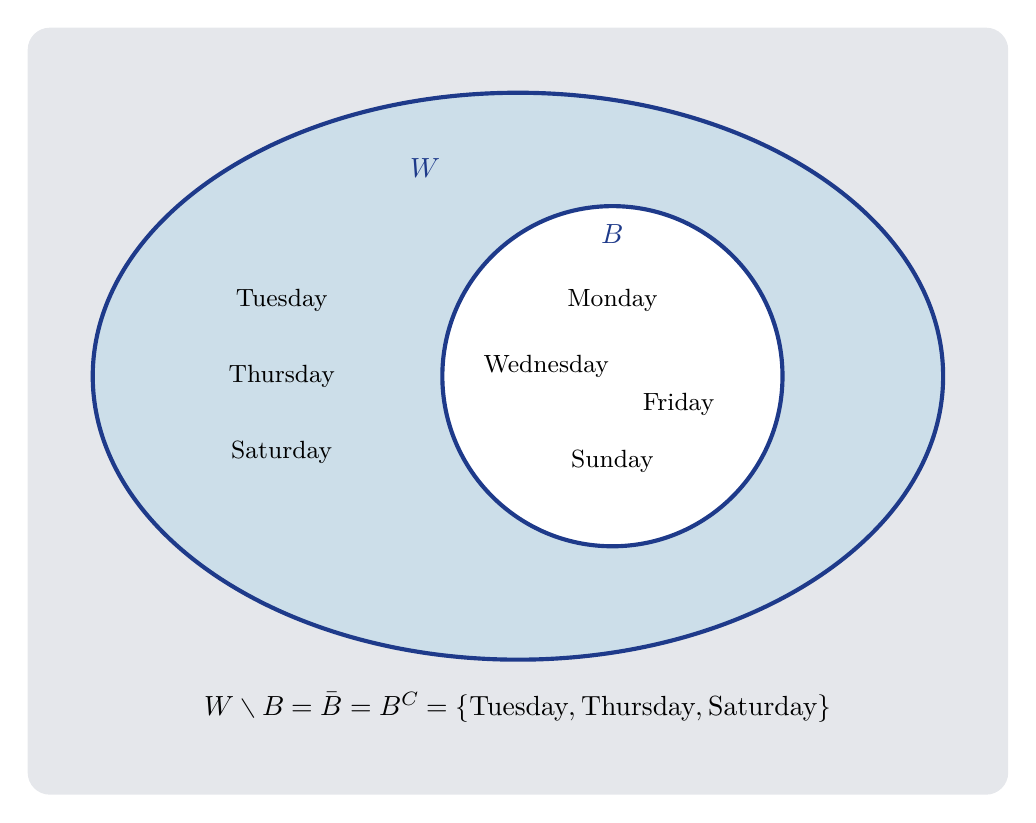
\begin{tikzpicture}[scale=1.2,
    show background rectangle,
    background rectangle/.style={fill=bgcolor, rounded corners=8pt},
    inner frame sep=0.8cm
]
  
  % Grundmenge W (große Ellipse)
  \fill[highlight] (0,0) ellipse (4.5cm and 3cm);
  
  % Menge B (Kreis) weiß übermalen
  \fill[bgcolor] (1,0) circle (1.8cm);
  
  % Menge B leicht füllen
  \fill[white] (1,0) circle (1.8cm);
  
  % Rahmen zeichnen
  \draw[thick, draw=myblue, line width=1.5pt] (0,0) ellipse (4.5cm and 3cm);
  \draw[thick, draw=myblue, line width=1.5pt] (1,0) circle (1.8cm);
  
  % Labels
  \node[myblue, font=\bfseries] at (-1.0,2.2) {$W$};
  \node[myblue, font=\bfseries] at (1,1.5) {$B$};
  
  % Elemente im Komplement W \ B (hervorgehoben)
  \node[font=\small] at (-2.5,0.8) {Tuesday};
  \node[font=\small] at (-2.5,0) {Thursday};
  \node[font=\small] at (-2.5,-0.8) {Saturday};
  
  % Elemente in B (nicht hervorgehoben)
  \node[font=\small] at (1,0.8) {Monday};
  \node[font=\small] at (0.3,0.1) {Wednesday};
  \node[font=\small] at (1.7,-0.3) {Friday};
  \node[font=\small] at (1,-0.9) {Sunday};
  
  % Formel
  \node at (0,-3.5) {$W \setminus B = \bar{B} = B^C = \{\text{Tuesday}, \text{Thursday}, \text{Saturday}\}$};
  
\end{tikzpicture}
\end{document}
